\documentclass[10pt]{article}
\usepackage[a4paper,bindingoffset=0.2in,left=0.25in,right=0.25in,top=0in,bottom=1in,footskip=.25in]{geometry}
\usepackage[utf8]{inputenc}
\usepackage[english]{babel}
\usepackage{amsmath}
\usepackage{mathptmx}
\usepackage[LY1]{fontenc}
\usepackage[utf8]{inputenc}
\usepackage{polski}
\usepackage[lf]{berenis}
\usepackage{xcolor}
\usepackage{color,soul}
\usepackage{graphicx}
\usepackage{subfig}
\graphicspath{ {./figs/} }
\title{Higgs CP}
\date{14.05.2020}

\begin{document}


\maketitle
\section{Introduction}
Elementary particles in Standard Model are divided for two groups, fermions and bosons, among others in second group are Higgs boson and Z boson. They both can decay in quite similar way. Right now this document shows histograms of their products (and with them some differences between Z and H decay). Data contains of events (which construction is discussed in next paragraph), for each particle file stored 1 milion of events.
\section{Example event record}
Each event consists of weight of an event, index of particle and its four vector. \newline
 TUPLE  1.558204  \newline
 2.816050  -4.370471  3.219078  6.115040 16 \newline
 9.202453  -12.449674  11.851361  19.497532 -211 \newline
 2.615191  -3.487638  3.806448  5.788791 111 \newline
 3.739119  20.131053  80.055826  82.632776 -16 \newline
 12.849713  76.012524  309.442587  318.900852 211 \newline
 1.817029  11.847960  46.472940  47.994043 111 \newline
Number in the first row is weight. Integers in last column are indexes of particles, rest numbers mean 4 vectors $(p_x,p_y,p_z,E)$.

\section{Histograms}
\begin{figure}[h] \centering
\subfloat[]{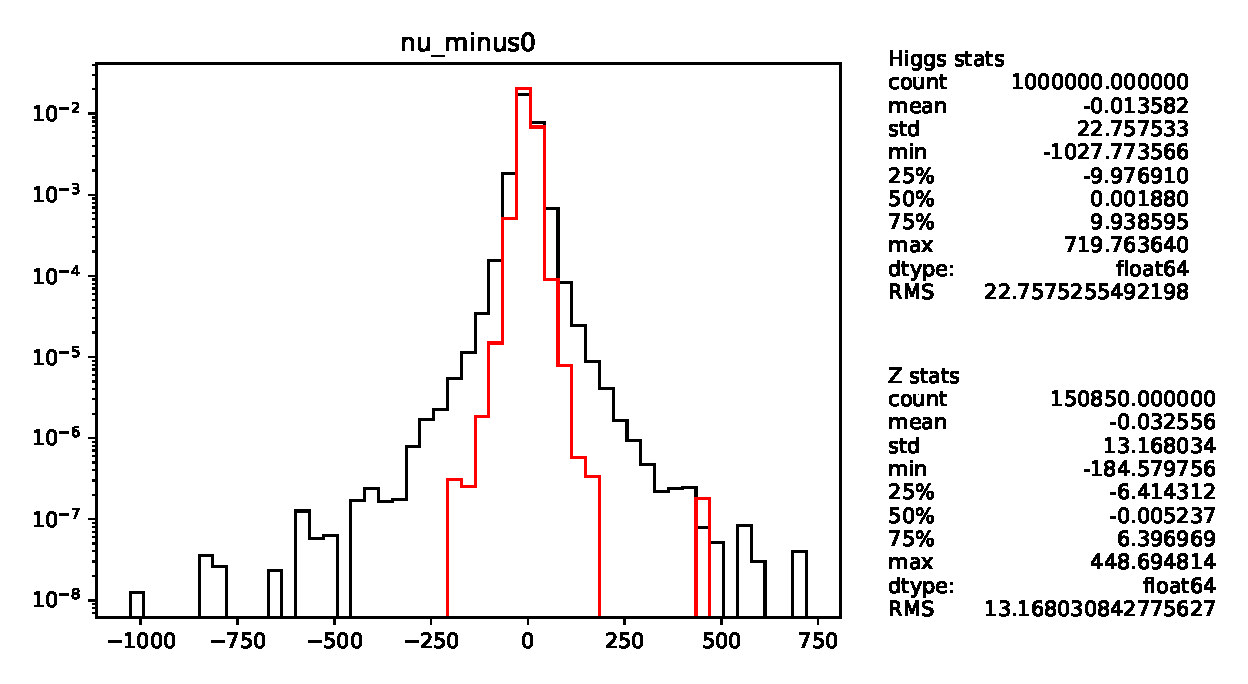
\includegraphics[width = 3.6in]{nu_minus0.eps}}
\subfloat[]{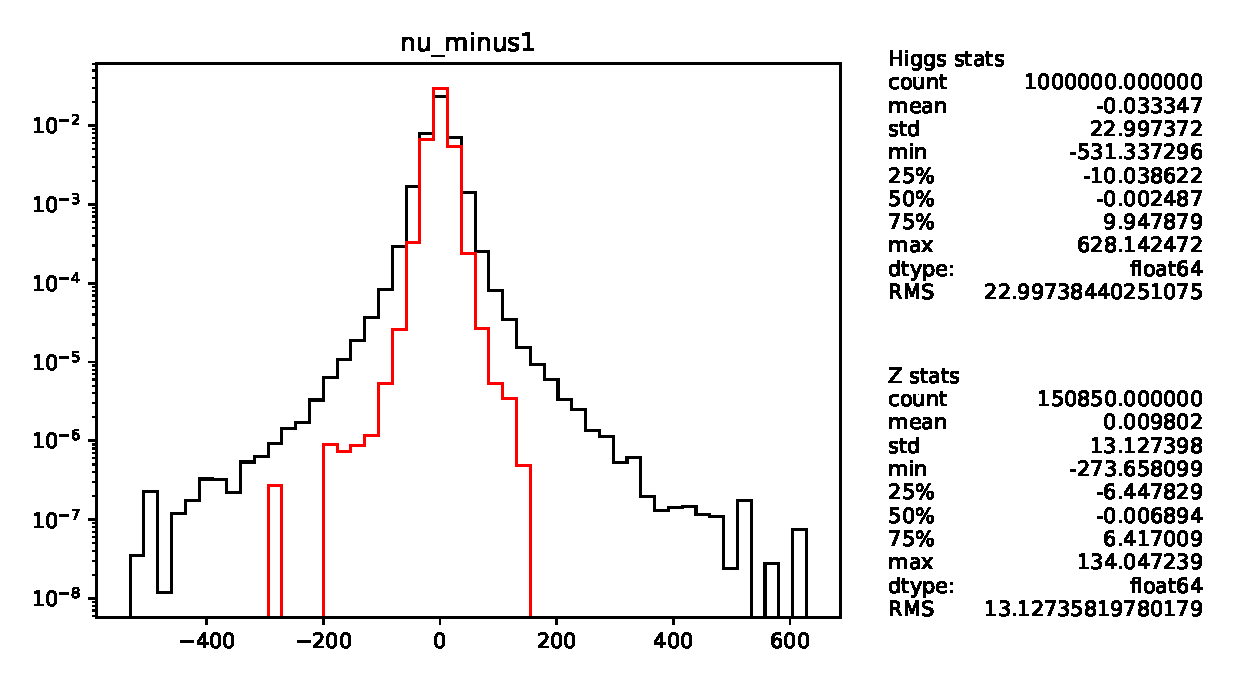
\includegraphics[width = 3.6in]{nu_minus1.eps}}
\newline
\subfloat[]{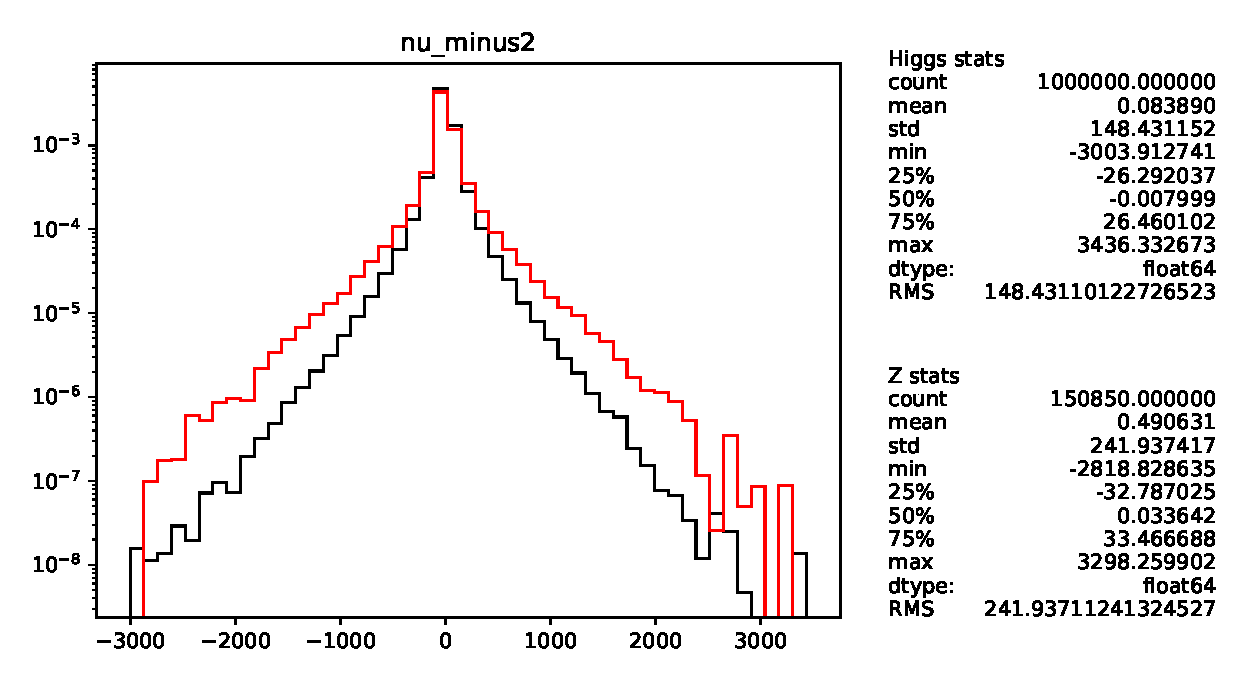
\includegraphics[width = 3.6in]{nu_minus2.eps}}
\subfloat[]{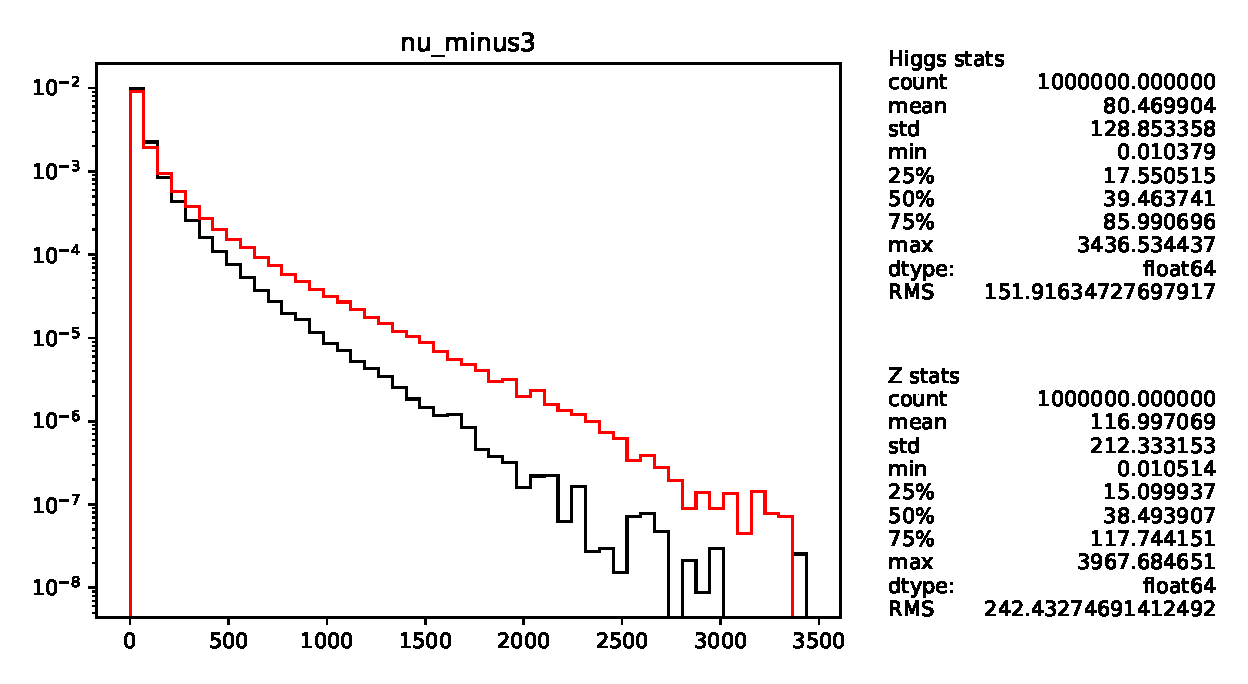
\includegraphics[width = 3.6in]{nu_minus3.eps}}
\newline
\subfloat[]{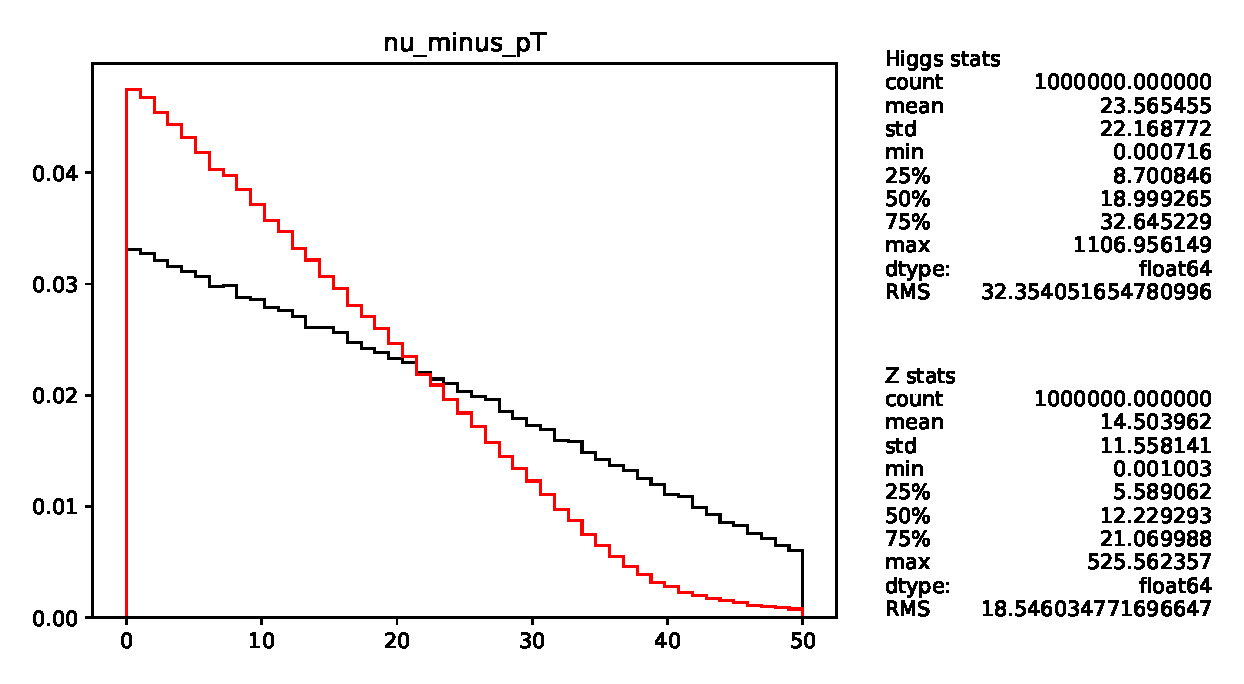
\includegraphics[width = 3.6in]{nu_minus_pT.eps}}
\caption{Histograms for each component of 4 vector $\nu_-$ and pT from H[black] and Z[red]}
\end{figure}
\begin{figure}[h] \centering
\subfloat[]{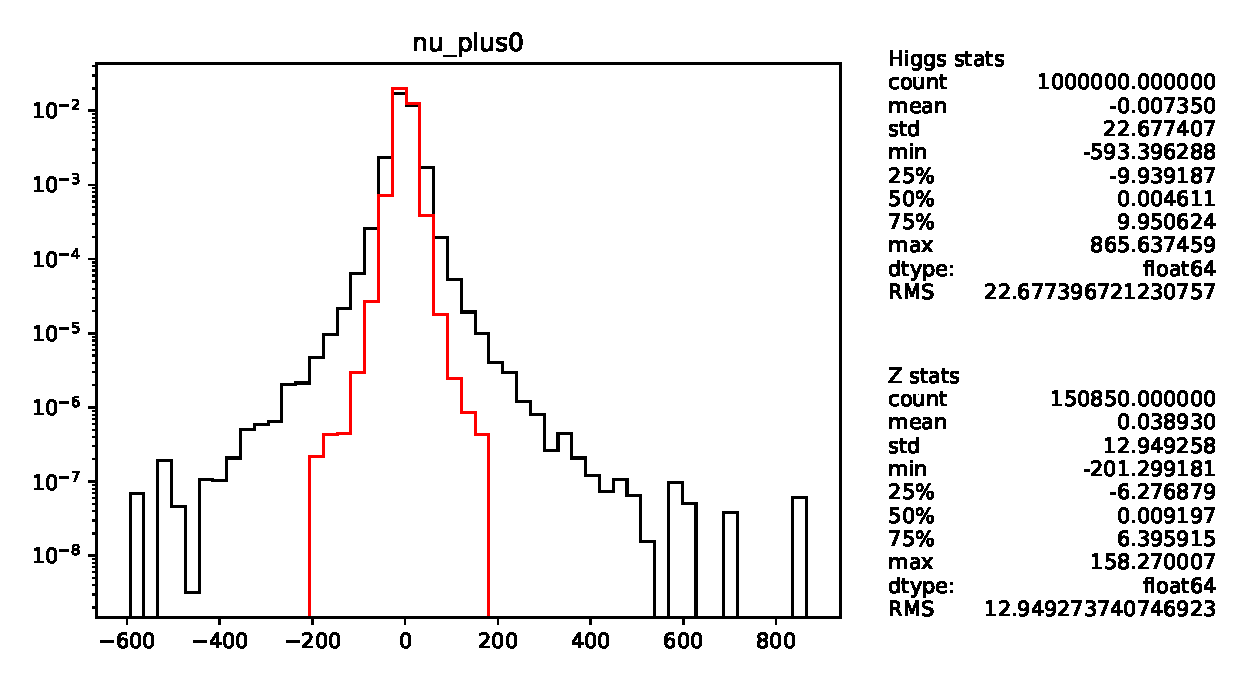
\includegraphics[width = 3.6in]{nu_plus0.eps}}
\subfloat[]{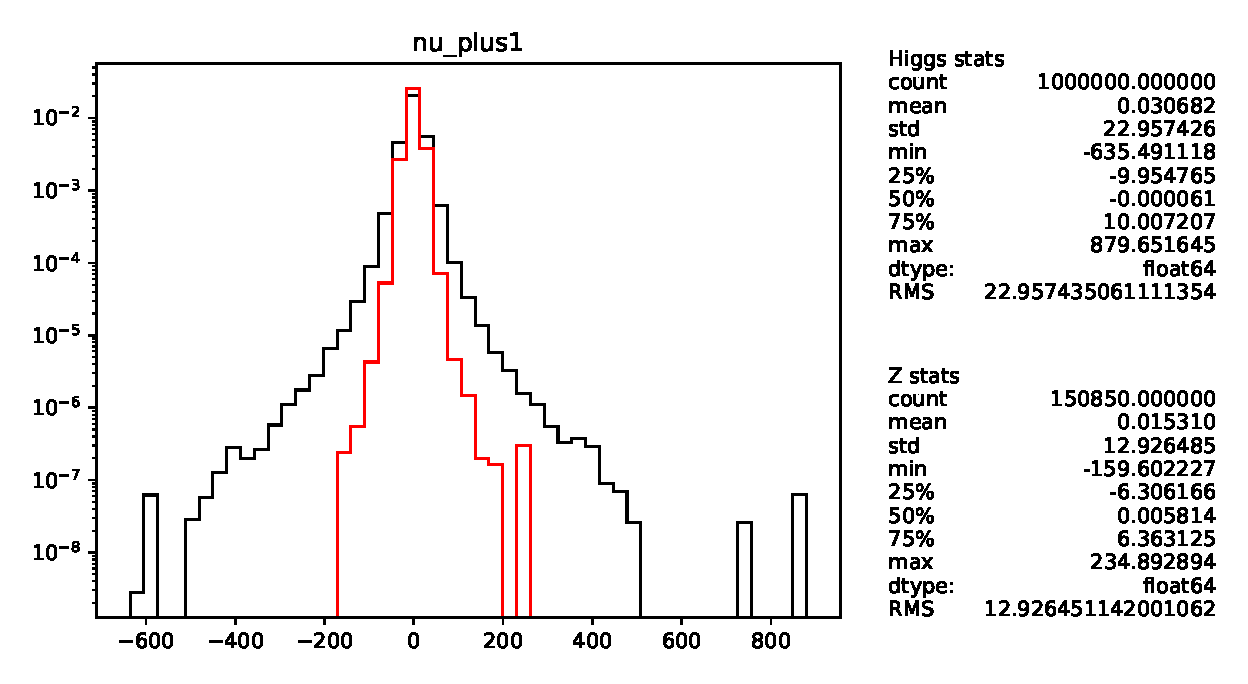
\includegraphics[width = 3.6in]{nu_plus1.eps}}
\newline
\subfloat[]{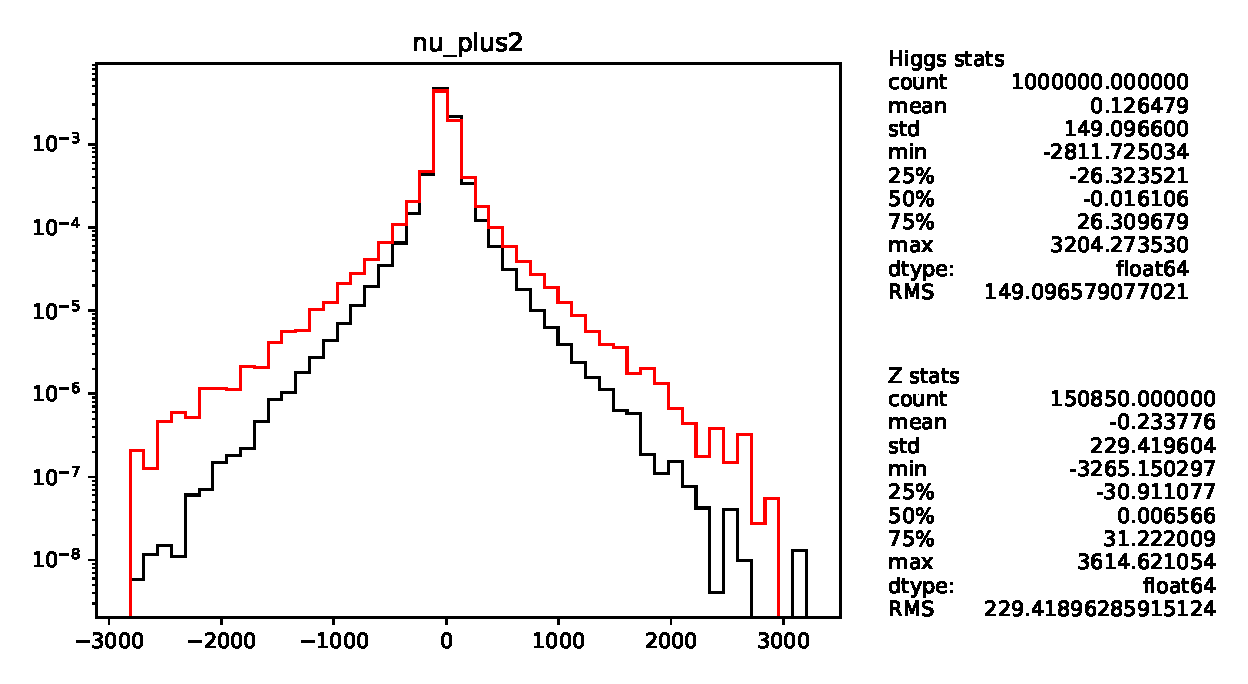
\includegraphics[width = 3.6in]{nu_plus2.eps}}
\subfloat[]{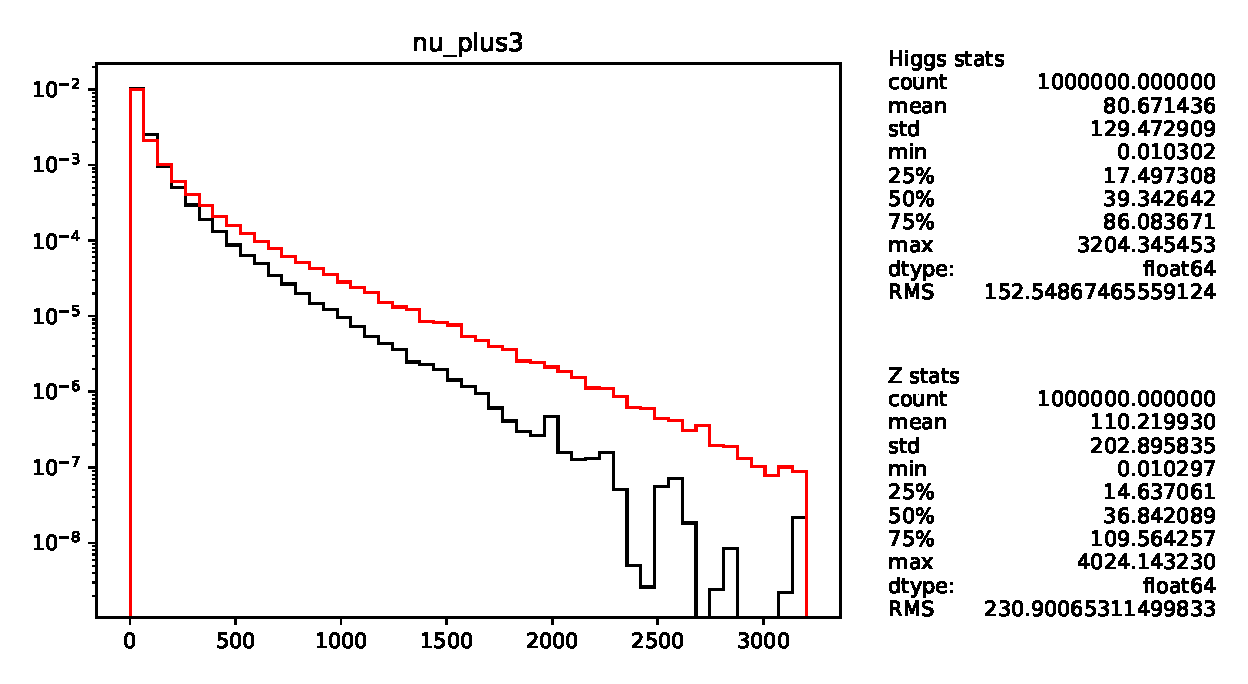
\includegraphics[width = 3.6in]{nu_plus3.eps}}
\newline
\subfloat[]{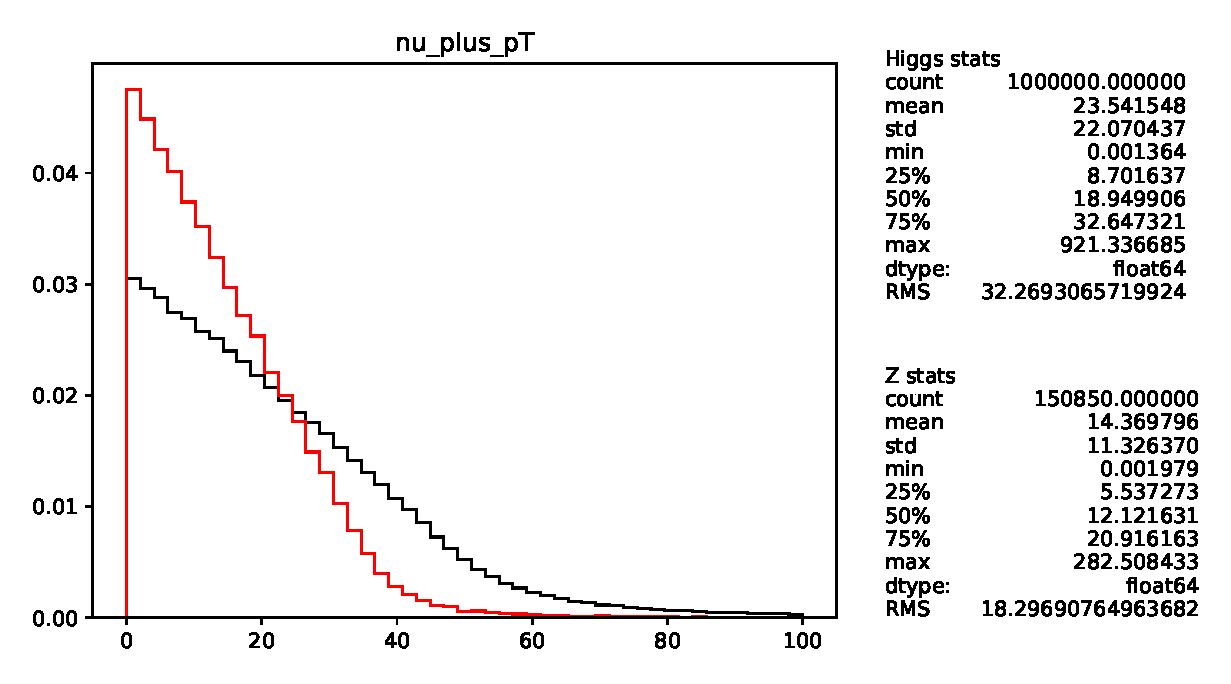
\includegraphics[width = 3.6in]{nu_plus_pT.eps}}
\caption{Histograms for each component of 4 vector $\nu_+$ and pT from H[black] and Z[red]}
\end{figure}
\begin{figure}[h] \centering
\subfloat[]{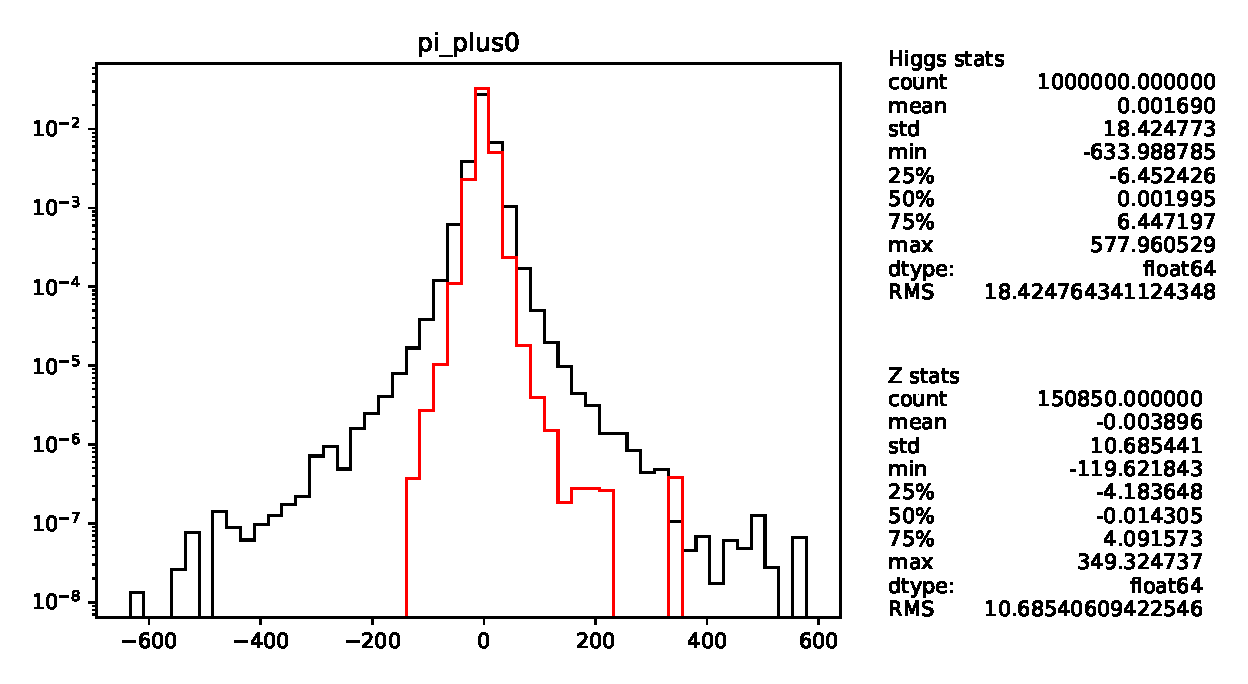
\includegraphics[width = 3.6in]{pi_plus0.eps}}
\subfloat[]{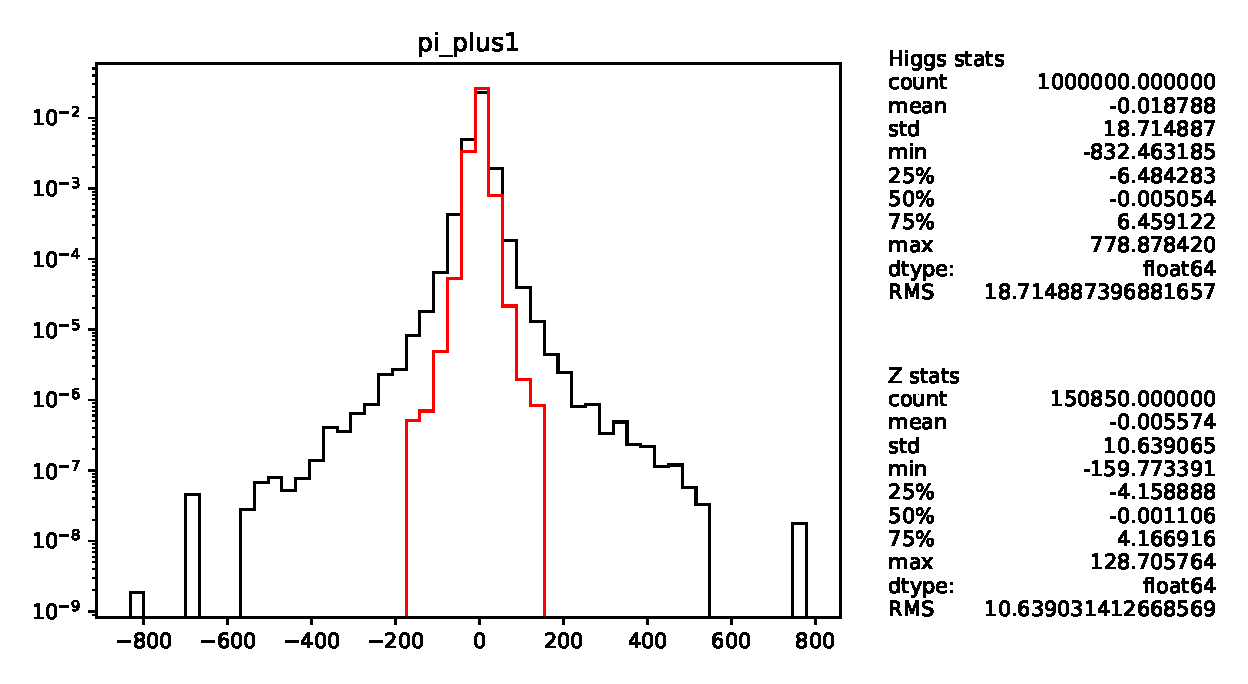
\includegraphics[width = 3.6in]{pi_plus1.eps}}
\newline
\subfloat[]{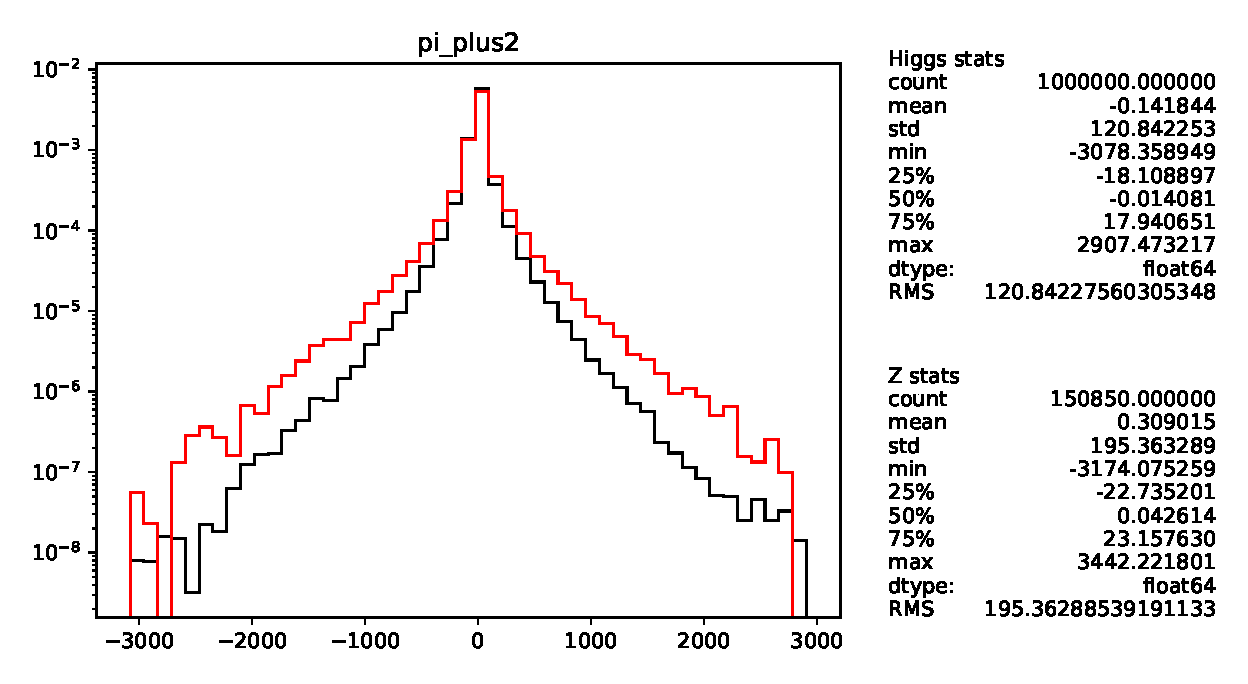
\includegraphics[width = 3.6in]{pi_plus2.eps}}
\subfloat[]{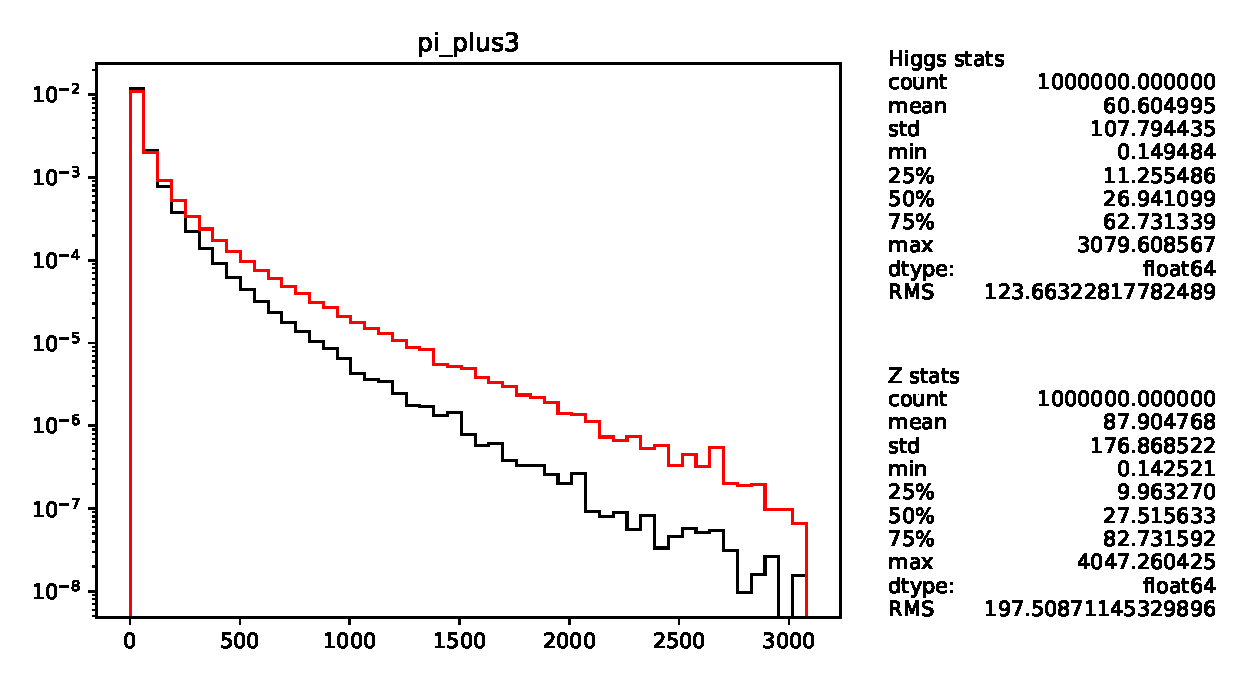
\includegraphics[width = 3.6in]{pi_plus3.eps}}
\newline
\subfloat[]{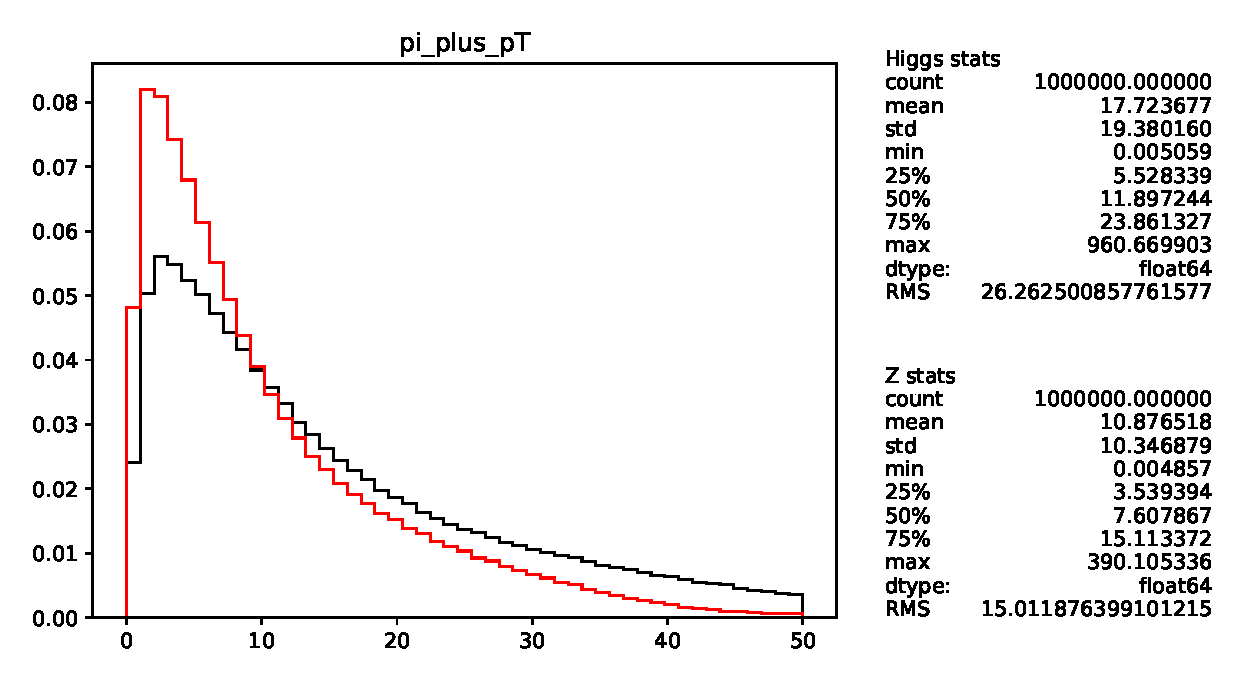
\includegraphics[width = 3.6in]{pi_plus_pT.eps}}
\caption{Histograms for each component of 4 vector $\pi_+$ and pT from H[black] and Z[red]}
\end{figure}
\begin{figure}[h] \centering
\subfloat[]{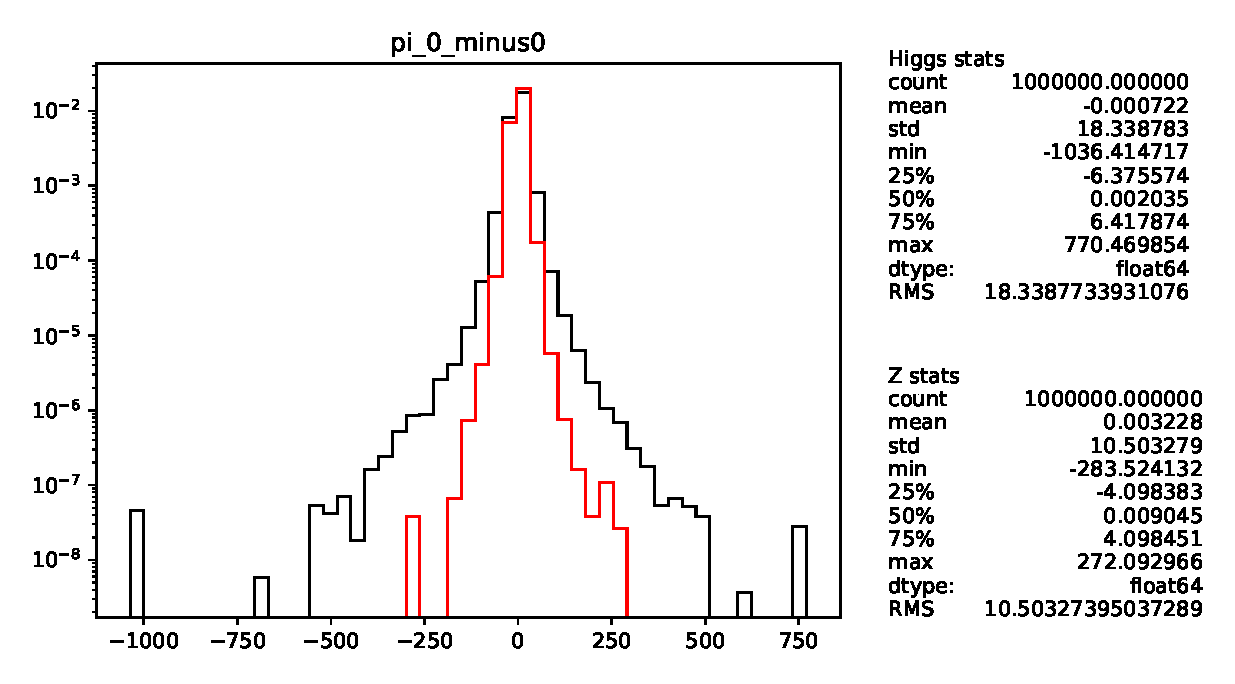
\includegraphics[width = 3.6in]{pi_0_minus0.eps}}
\subfloat[]{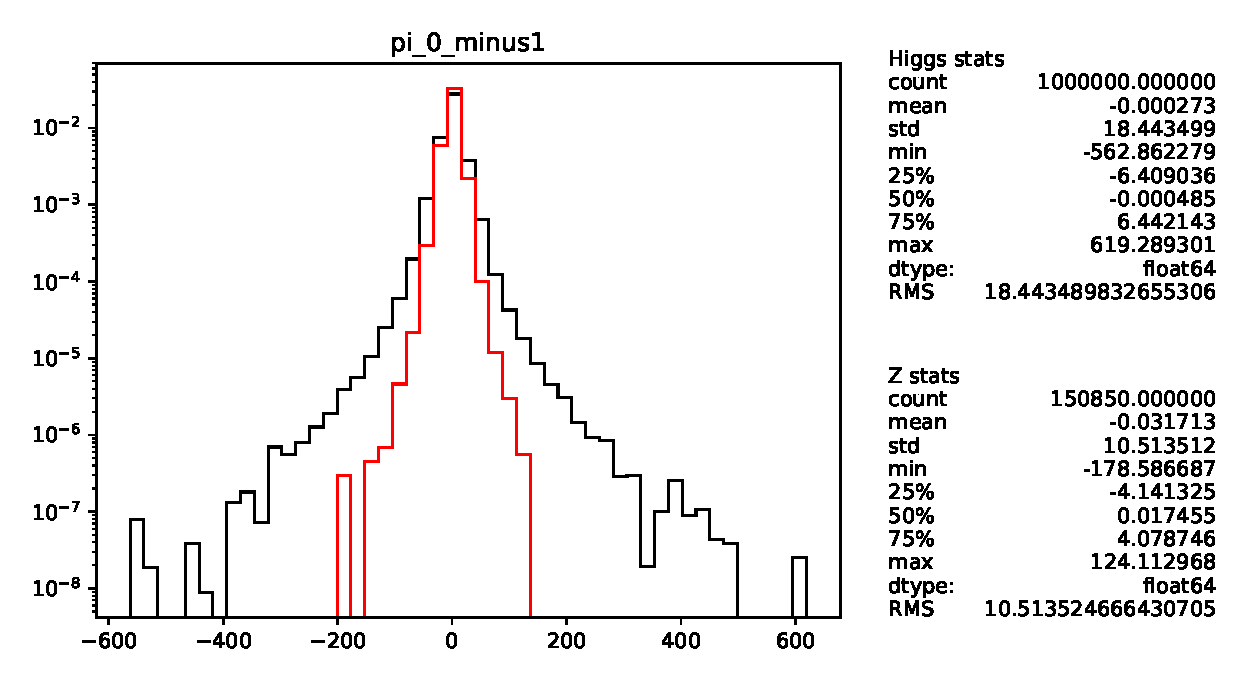
\includegraphics[width = 3.6in]{pi_0_minus1.eps}}
\newline
\subfloat[]{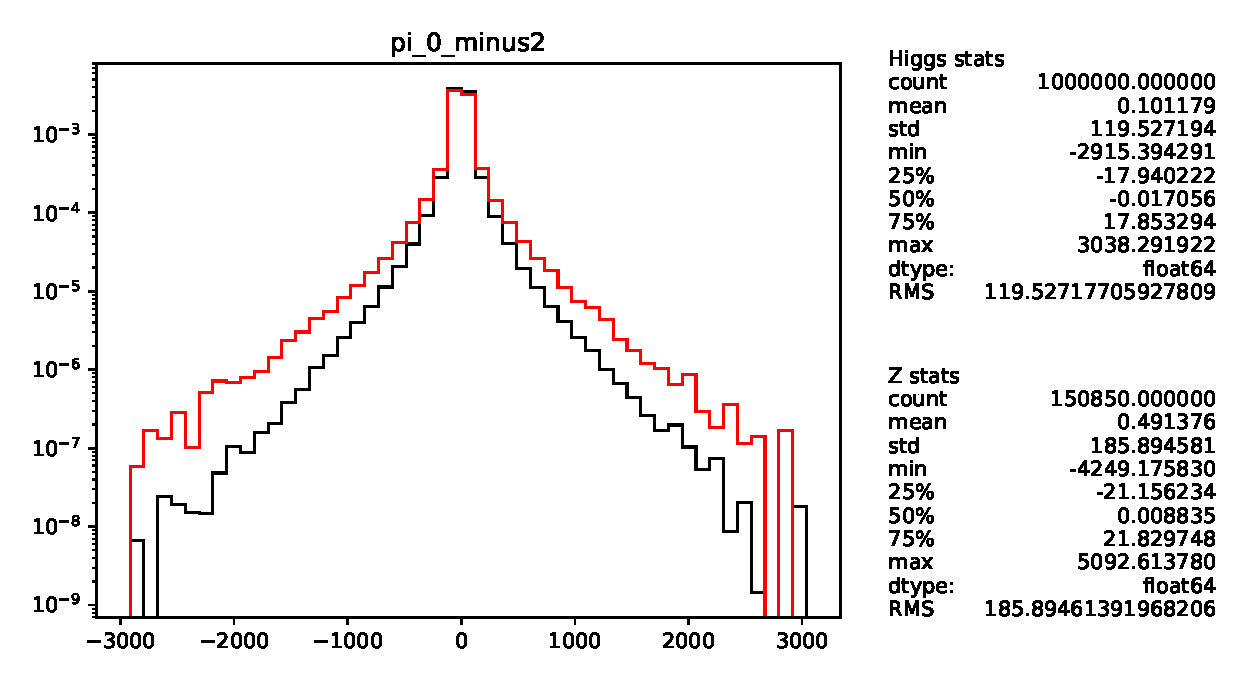
\includegraphics[width = 3.6in]{pi_0_minus2.eps}}
\subfloat[]{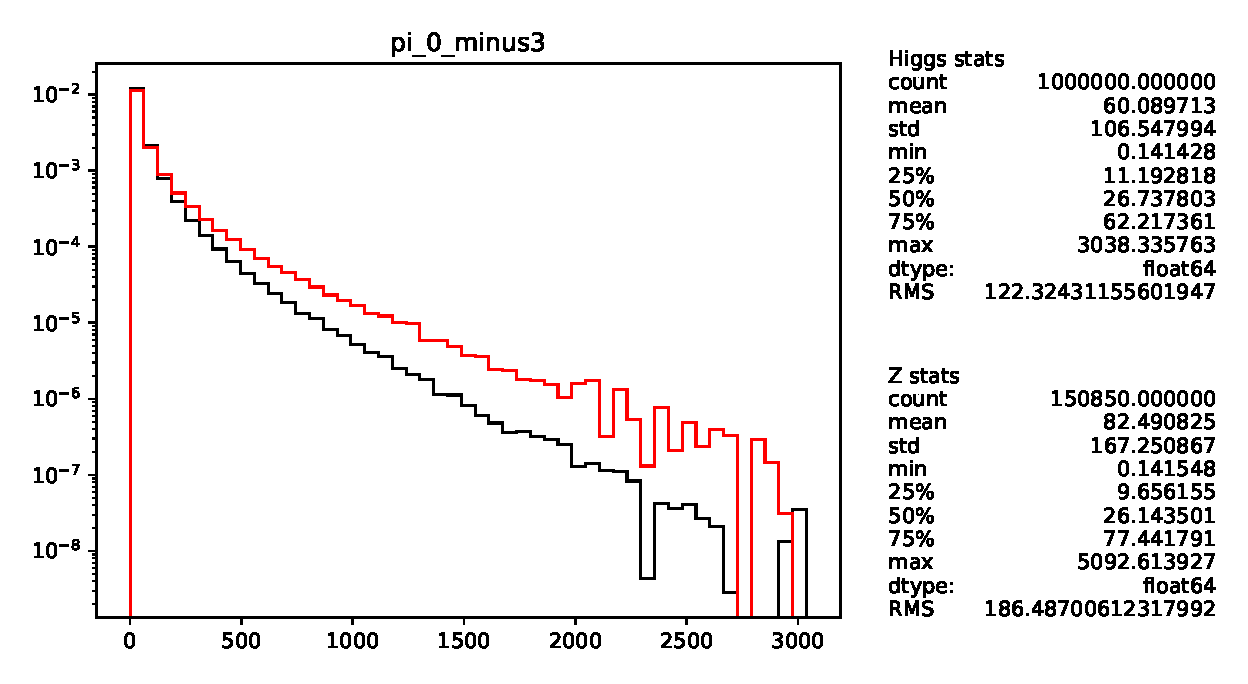
\includegraphics[width = 3.6in]{pi_0_minus3.eps}}
\newline
\subfloat[]{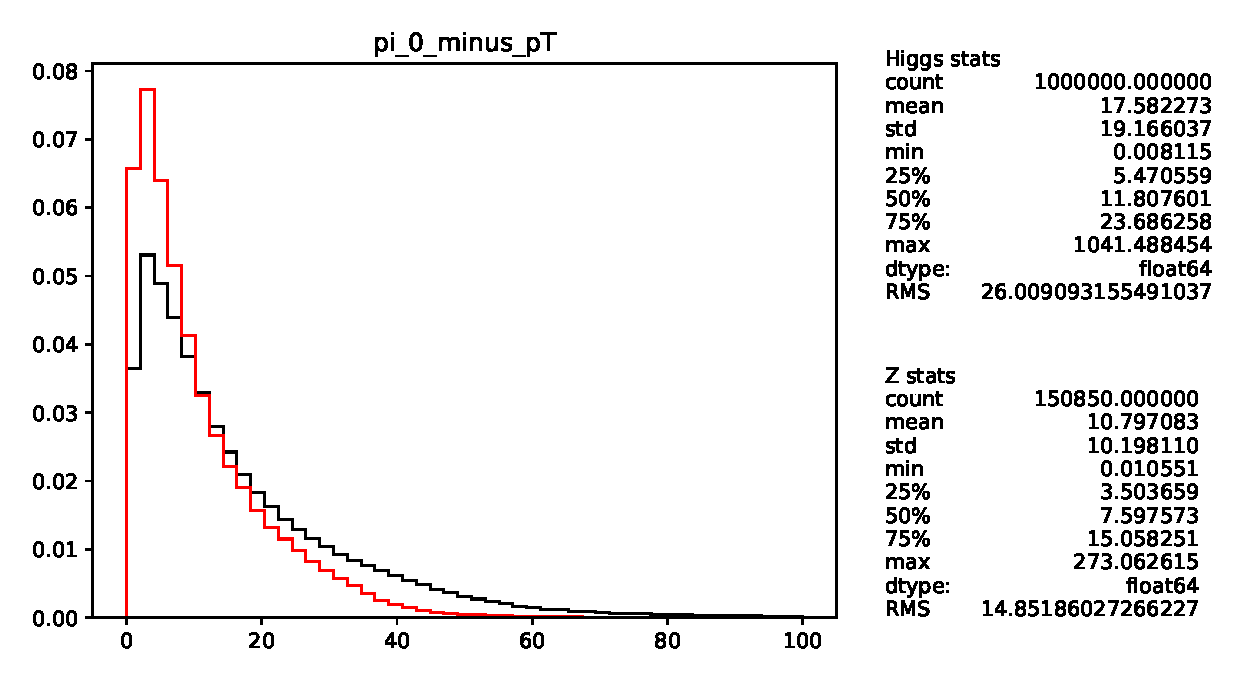
\includegraphics[width = 3.6in]{pi_0_minus_pT.eps}}
\caption{Histograms for each component of 4 vector $\pi_{0-}$ and pT from H[black] and Z[red]}
\end{figure}
\begin{figure}[h] \centering
\subfloat[]{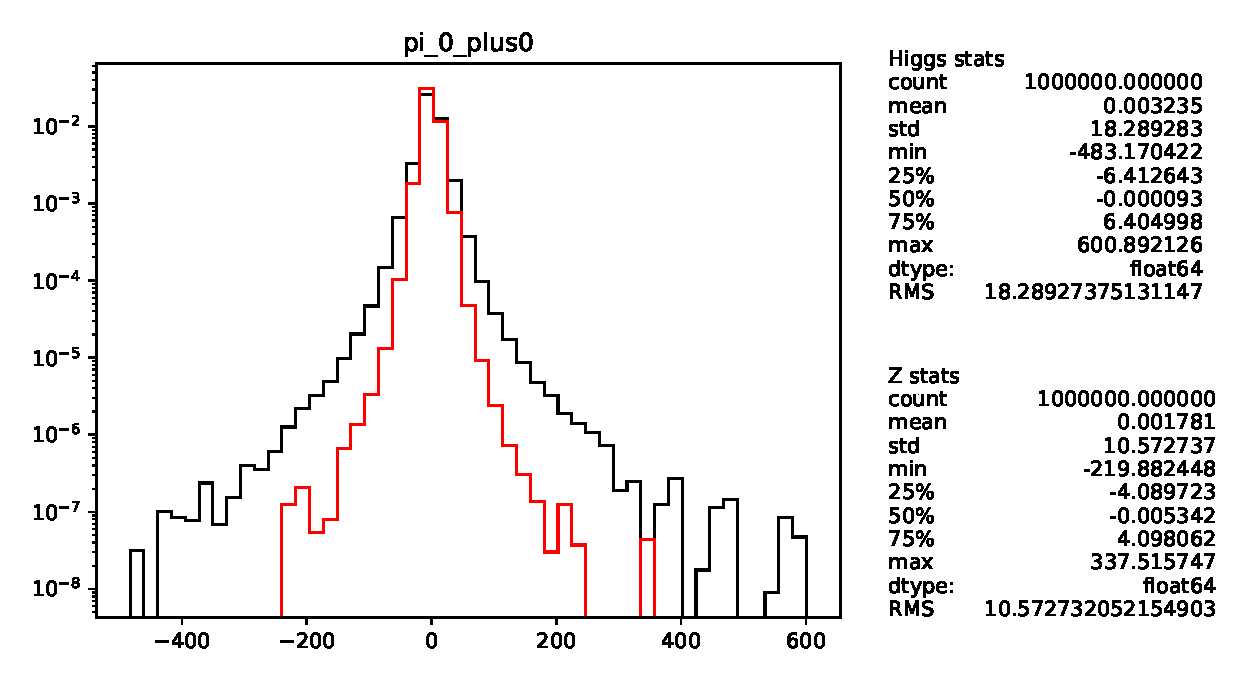
\includegraphics[width = 3.6in]{pi_0_plus0.eps}}
\subfloat[]{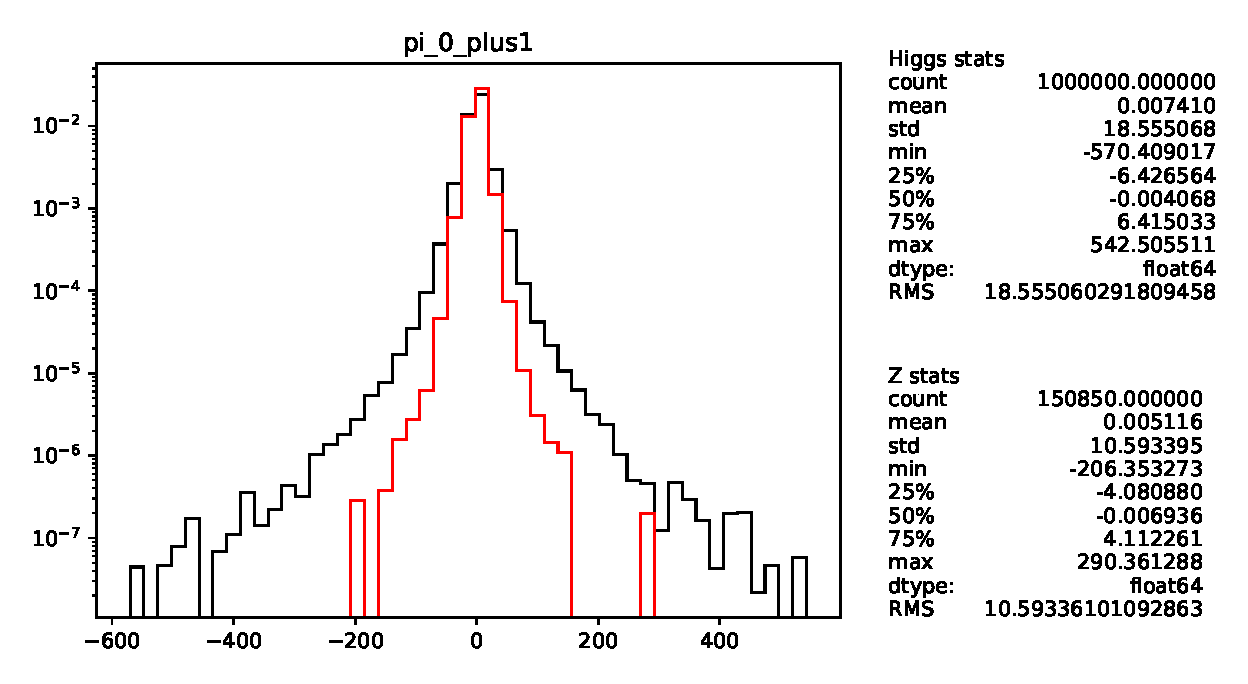
\includegraphics[width = 3.6in]{pi_0_plus1.eps}}
\newline
\subfloat[]{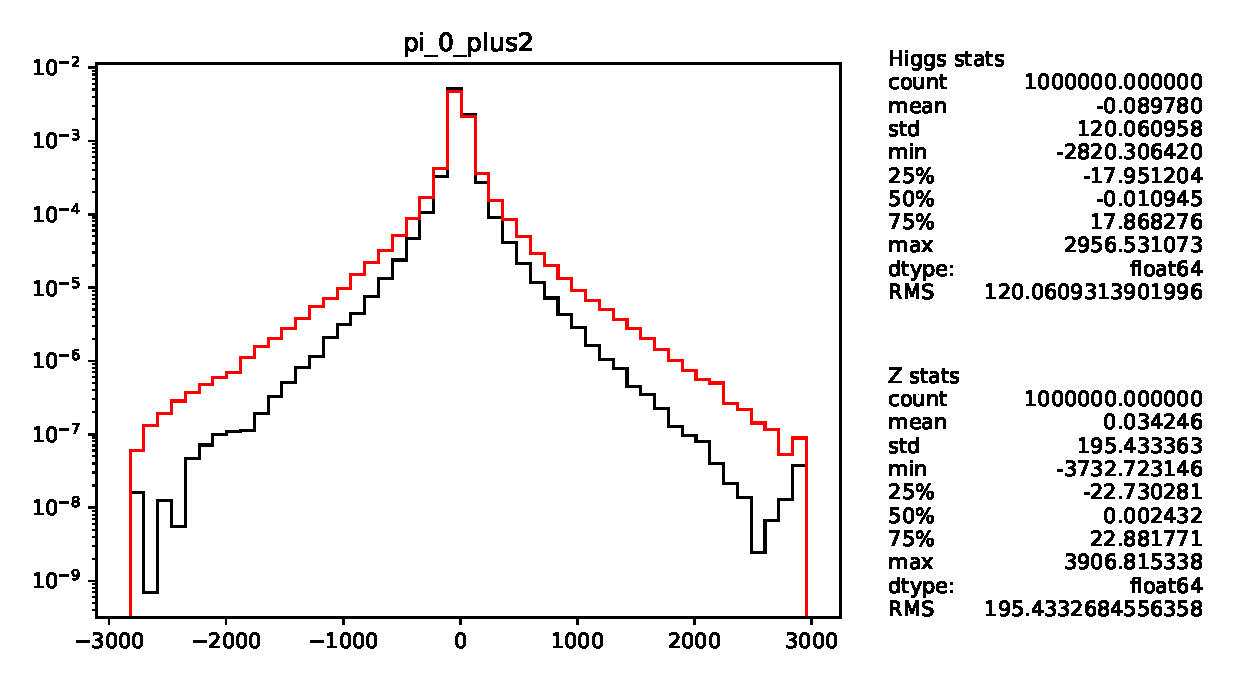
\includegraphics[width = 3.6in]{pi_0_plus2.eps}}
\subfloat[]{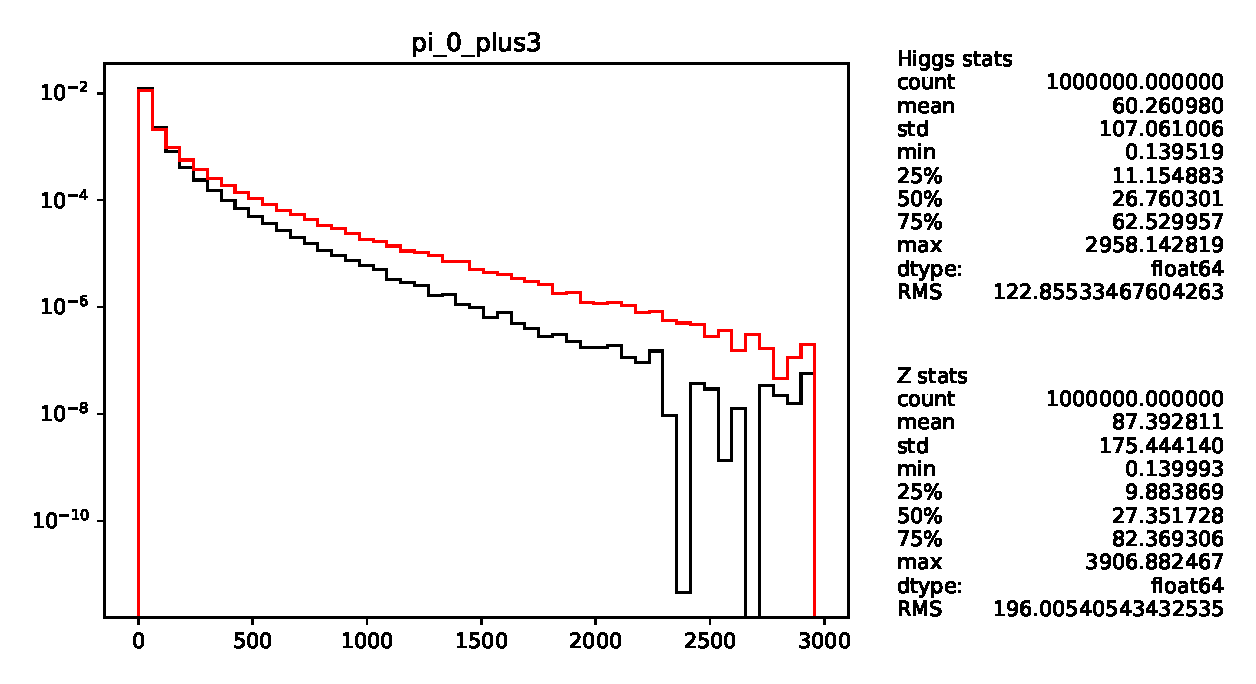
\includegraphics[width = 3.6in]{pi_0_plus3.eps}}
\newline
\subfloat[]{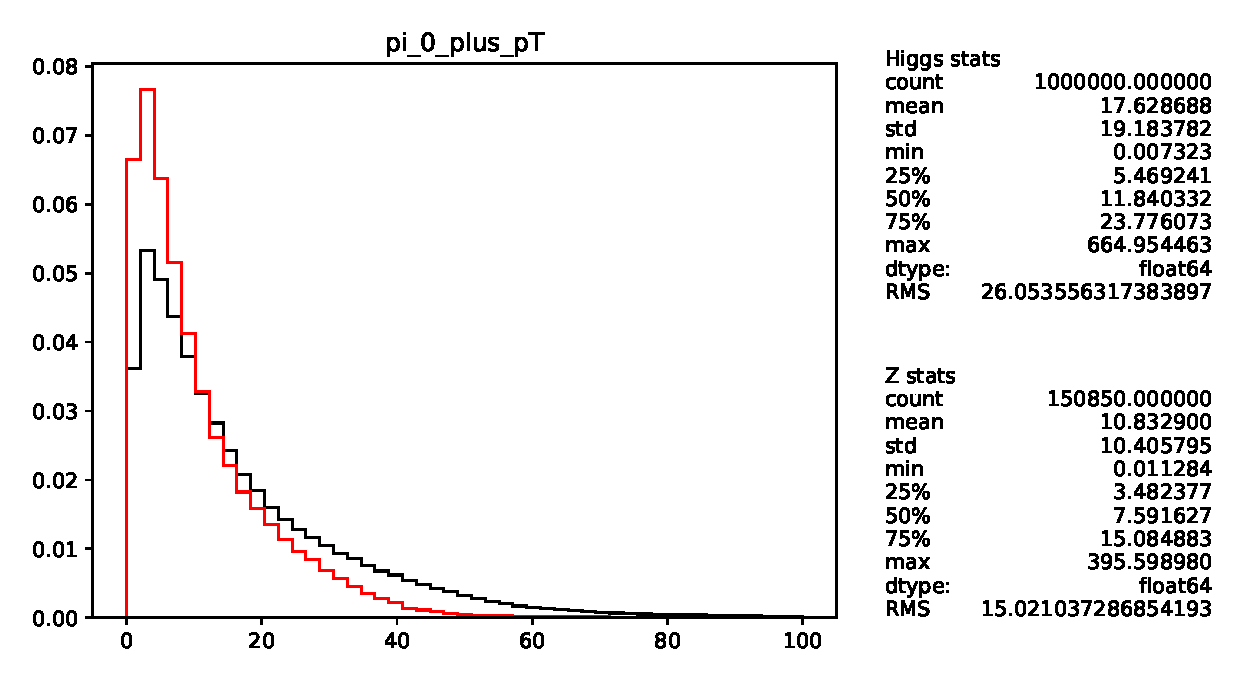
\includegraphics[width = 3.6in]{pi_0_plus_pT.eps}}
\caption{Histograms for each component of 4 vector $\pi_{0+}$ and pT from H[black] and Z[red]}
\end{figure}
\begin{figure}[h] \centering
\subfloat[]{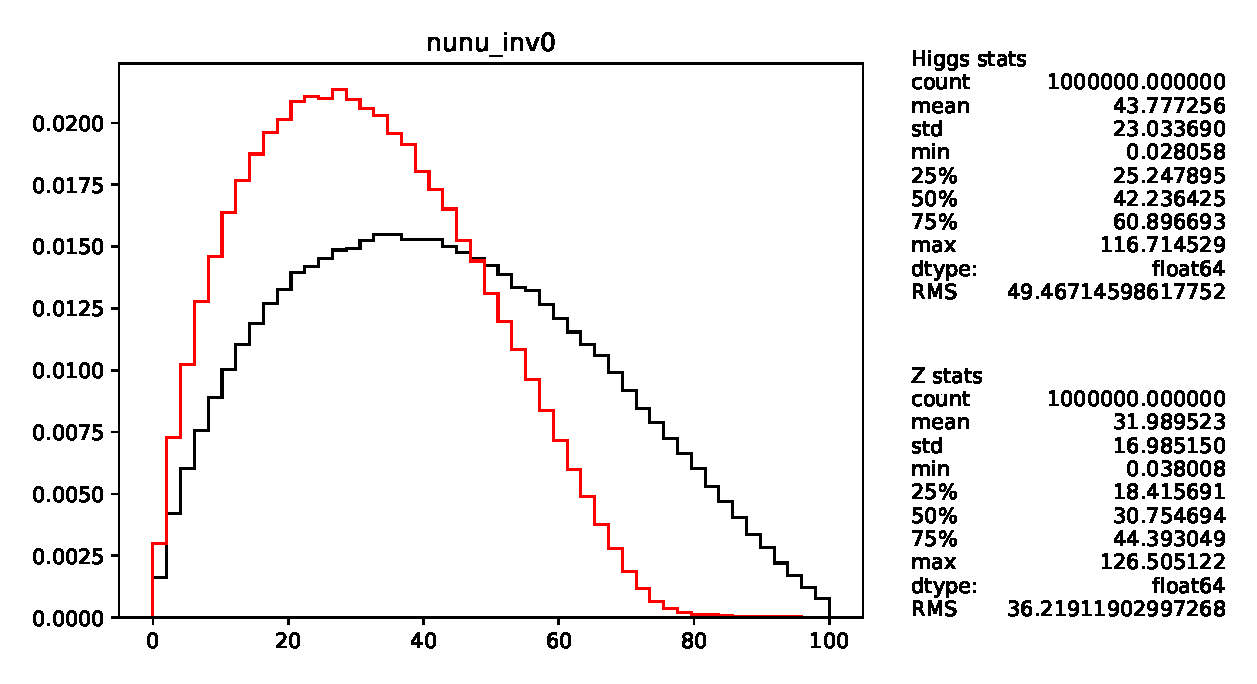
\includegraphics[width = 3.6in]{nunu_inv0.eps}}
\subfloat[]{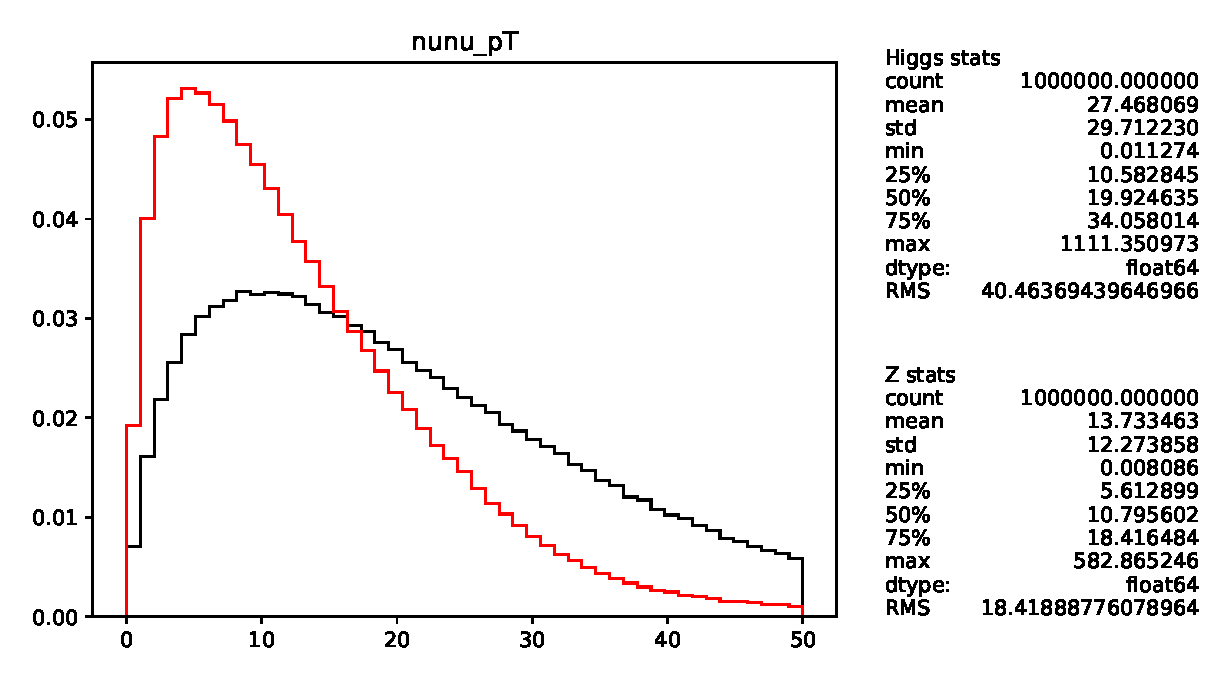
\includegraphics[width = 3.6in]{nunu_pT.eps}}
\caption{Histograms for $\nu \nu$ event (invariant mass and pT) for H[black] and Z[red]}
\end{figure}
\begin{figure}[h] \centering
\subfloat[]{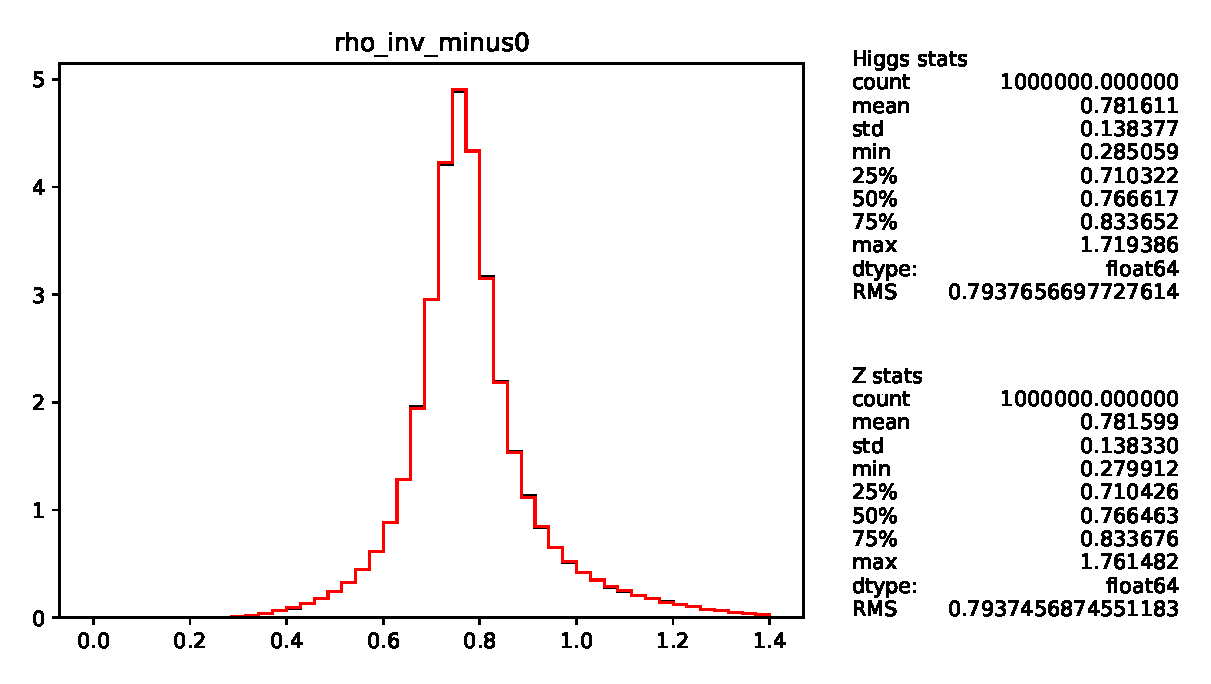
\includegraphics[width = 3.6in]{rho_inv_minus0.eps}}
\subfloat[]{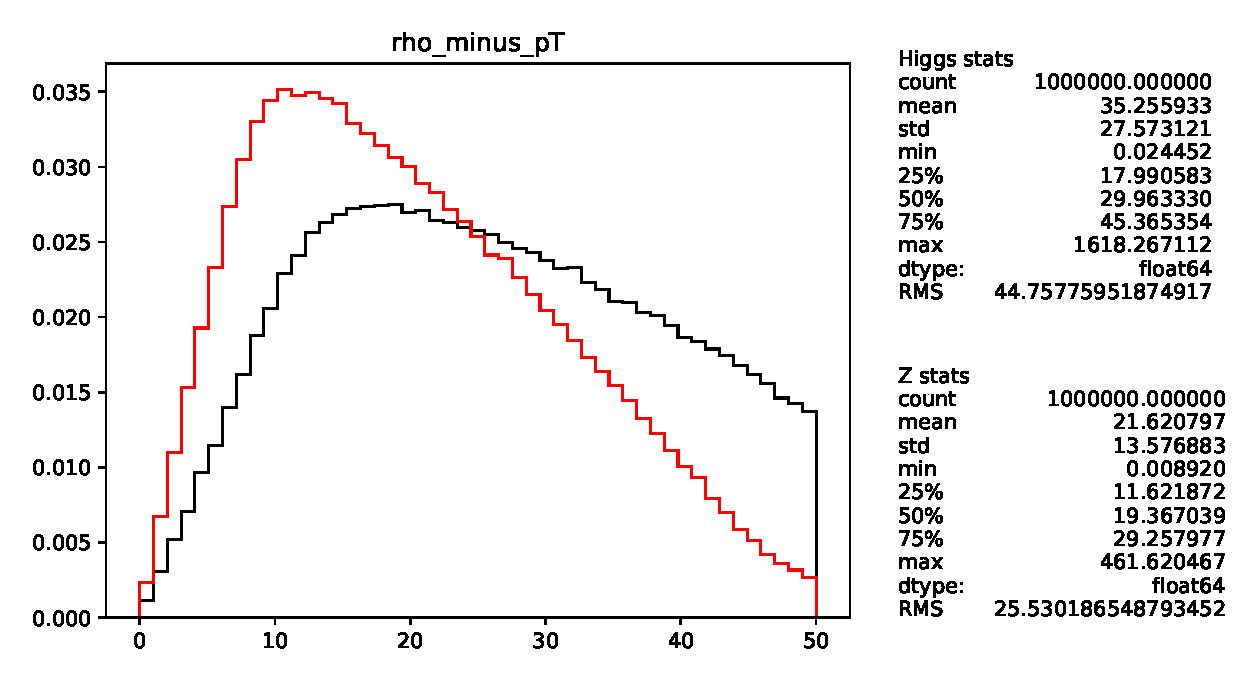
\includegraphics[width = 3.6in]{rho_minus_pT.eps}}
\caption{Histograms for $\rho _-$ event (invariant mass and pT) for H[black] and Z[red]}
\end{figure}
\begin{figure}[h] \centering
\subfloat[]{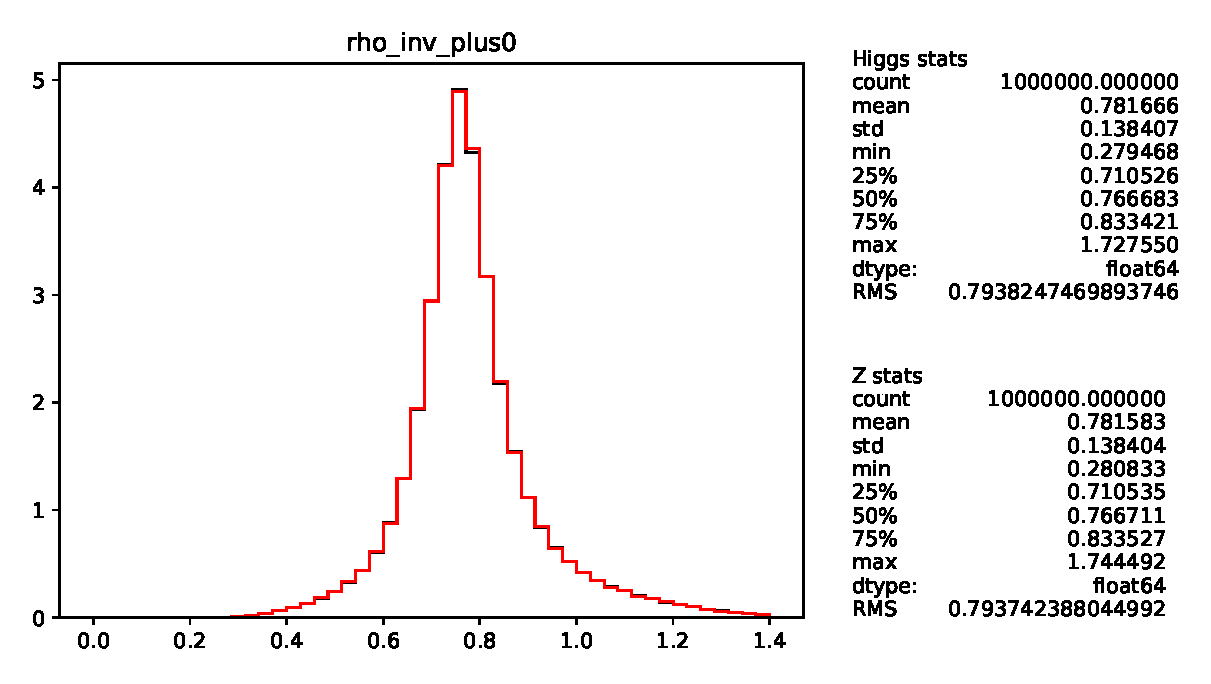
\includegraphics[width = 3.6in]{rho_inv_plus0.eps}}
\subfloat[]{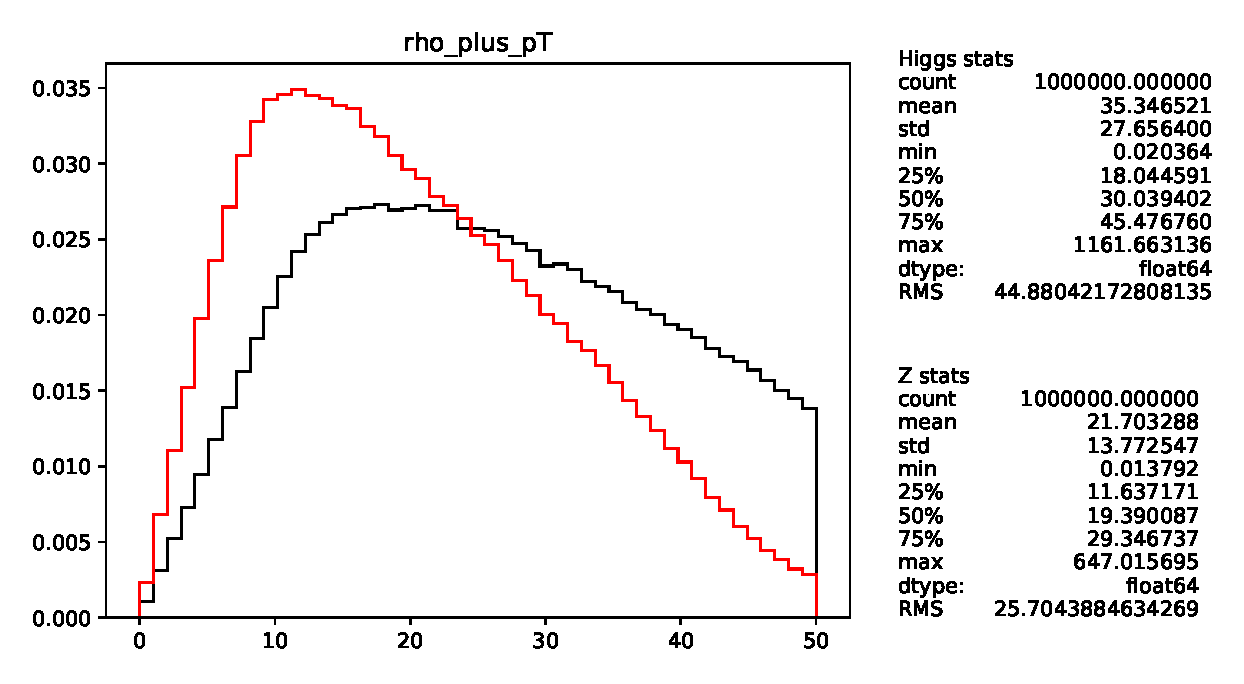
\includegraphics[width = 3.6in]{rho_plus_pT.eps}}
\caption{Histograms for $\rho _+$ event (invariant mass and pT) for H[black] and Z[red]}
\end{figure}
\begin{figure}[h] \centering
\subfloat[]{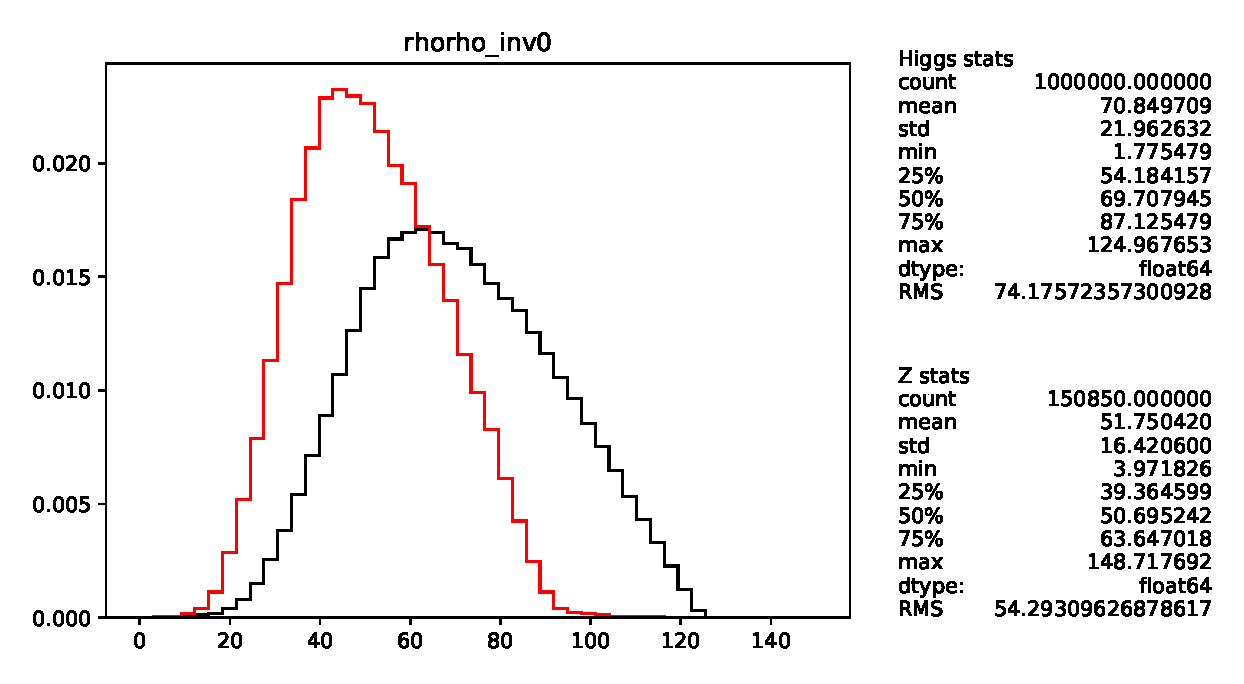
\includegraphics[width = 3.6in]{rhorho_inv0.eps}}
\subfloat[]{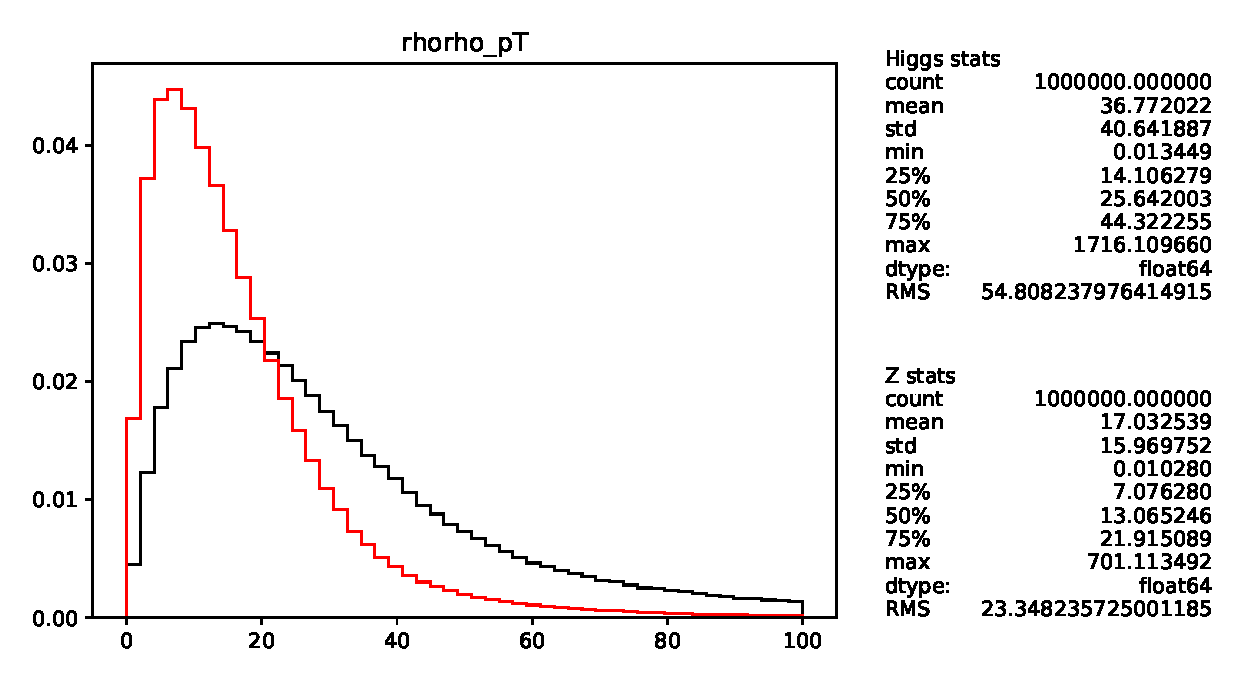
\includegraphics[width = 3.6in]{rhorho_pT.eps}}
\caption{Histograms for $\rho \rho$ event (invariant mass and pT) for H[black] and Z[red]}
\end{figure}
\begin{figure}[h] \centering
\subfloat[]{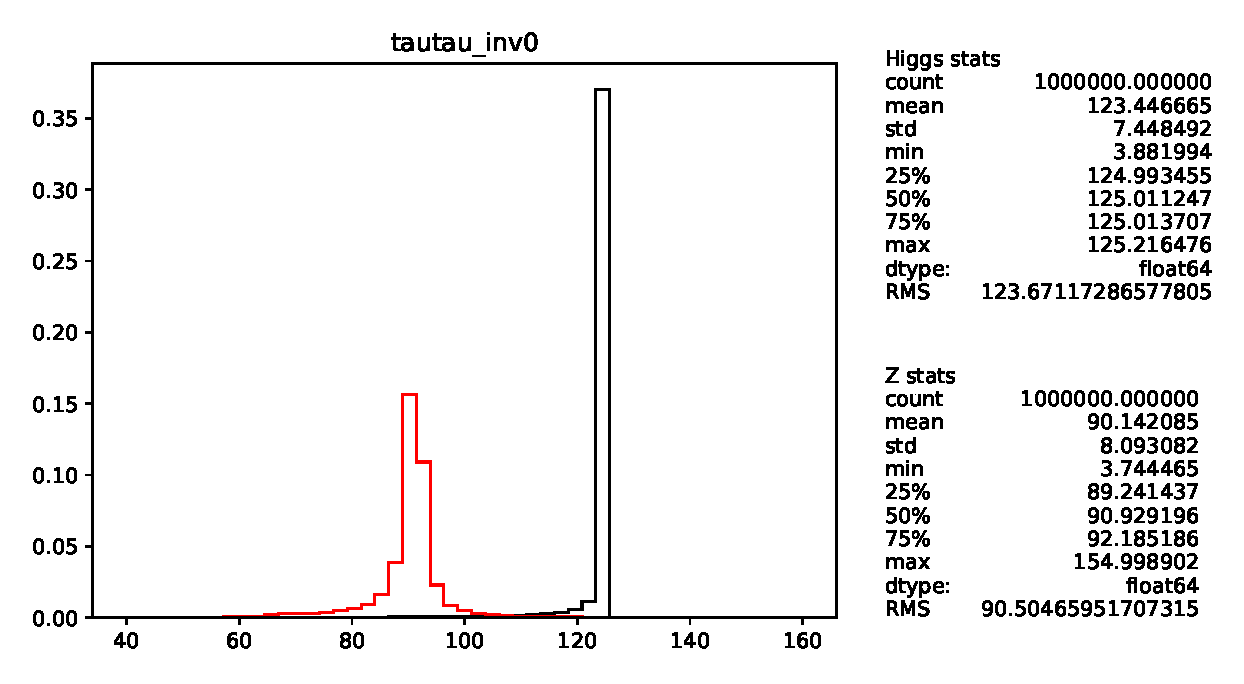
\includegraphics[width = 3.6in]{tautau_inv0.eps}}
\subfloat[]{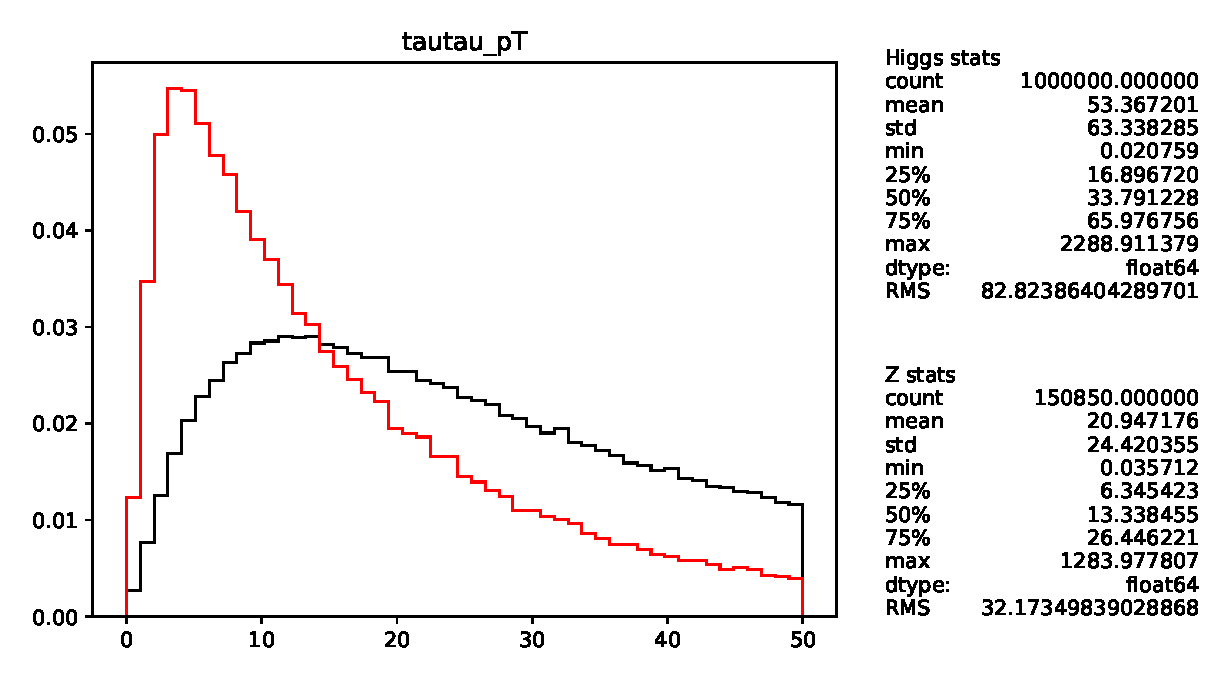
\includegraphics[width = 3.6in]{tautau_pT.eps}}
\caption{Histograms for $\tau \tau$ event (invariant mass and pT) for H[black] and Z[red]}
\end{figure}
\begin{figure}[h] \centering
\subfloat[]{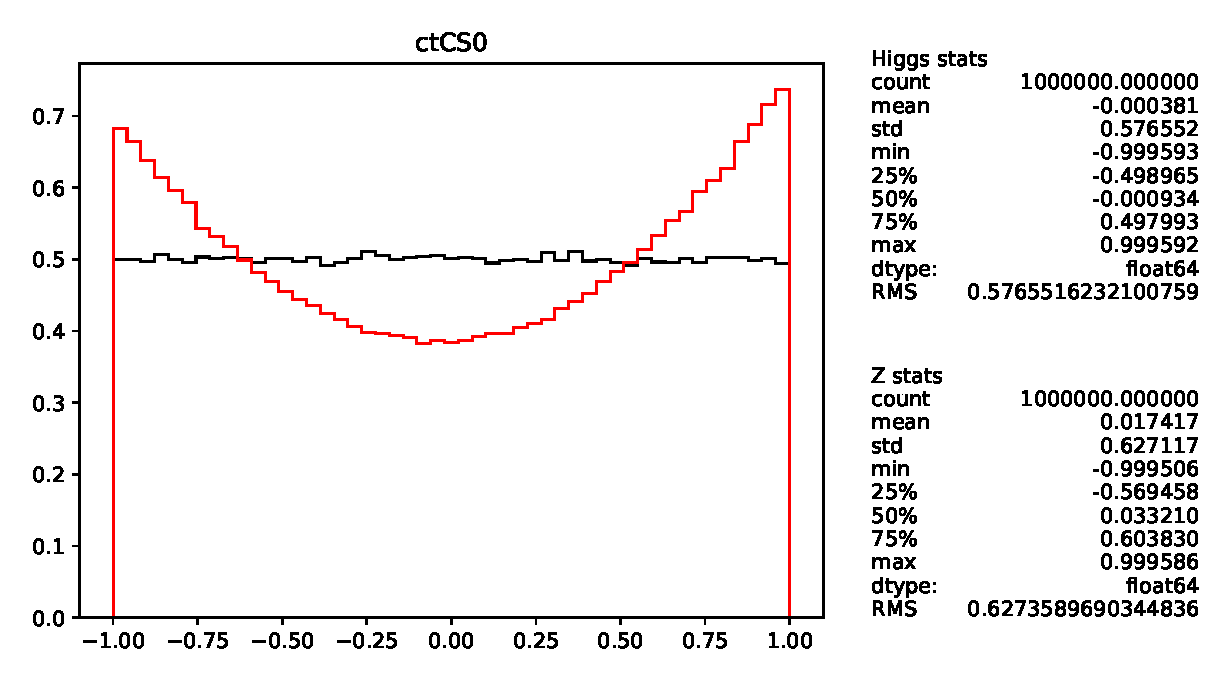
\includegraphics[width = 3.6in]{ctCS0.eps}}
\caption{Histogram of $Cos(\theta _{CS})$ value}
\end{figure}
\end{document}
